\section{Problem Statement}

\begin{definition}[Dynamic heterogeneous information network]
A dynamic heterogeneous information network is defined as a directed graph $G$ = ($V$, $E$), where $V$ and $E$ are set of nodes and edges of different types, and edges have timestamps. $\Box$ \amin{double check with HIN defiition}
\end{definition}

\begin{example}
The DBLP bibliographic network\footnote{\url{http://dblp.uni-trier.de/db/}} is a dynamic heterogeneous information network, containing different types of nodes such as papers, authors, topics, and publication venues, with publication links associated with date. Twitter social network is another example with nodes of types posted tweets, users, topics, and hashtags and time window associated with these tweets. $\Box$
\end{example}

In the context of a heterogenous network, a \textit{relation} can be in the form of a \textit{direct link} or an \textit{indirect link}, where an indirect link is a sequence of direct links in the network. Thus, two nodes might not be directly connected, however they might be connected considering the semantic of a sequence of links of different types. In this work, we use the terms \textit{relationship prediction} and \textit{link prediction} interchangeably referring to predicting whether two nodes will be connected in future via a sequence of relations in the graph. Note that the length of a sequence can be greater than or equal to one. For instance in a bibliographic network a direct link exist between an author and a paper he wrote, and an indirect link exist between him and his co-authors through the paper, which they wrote together.

\begin{definition}[\textbf{Relationship prediction problem}]\label{problemdef}
Given a dynamic heterogeneous information network $G$ at time $t$, and a target relation type $R$, we aim to predict the existence of a relation of type $R$ between two given nodes at time $t+1$. $\Box$
 \end{definition}

In order to better understand different types of nodes and their relation in a network, the concept of \textit{network schema} \cite{sun2011pathsim} is used. The network schema is a meta structure graph that summarizes a heterogeneous information network and is formally defined as bellow.

\begin{definition}[Network schema]
For a heterogeneous network $G=(V,E)$, the network schema $S_G=\mathcal{(A,R)}$ is a directed meta graph where $\mathcal{A}$ is the set of node types in $V$ and $\mathcal{R}$ is the set of relation types in $E$.  $\Box$
\end{definition}

\begin{example}
Figure \ref{schema} shows the network schema for the DBLP bibliographic network with $\mathcal{A}$=\{\textit{Author}, \textit{Paper}, \textit{Venue}, \textit{Topic}\}. $\Box$
\end{example}

In this paper, we refer to different types of nodes in the DBLP bibliographic network with abbreviations $P$ for paper, $A$ for author, $T$ for topic, and $V$ for venue. 

\begin{figure}[t]
  \centering
      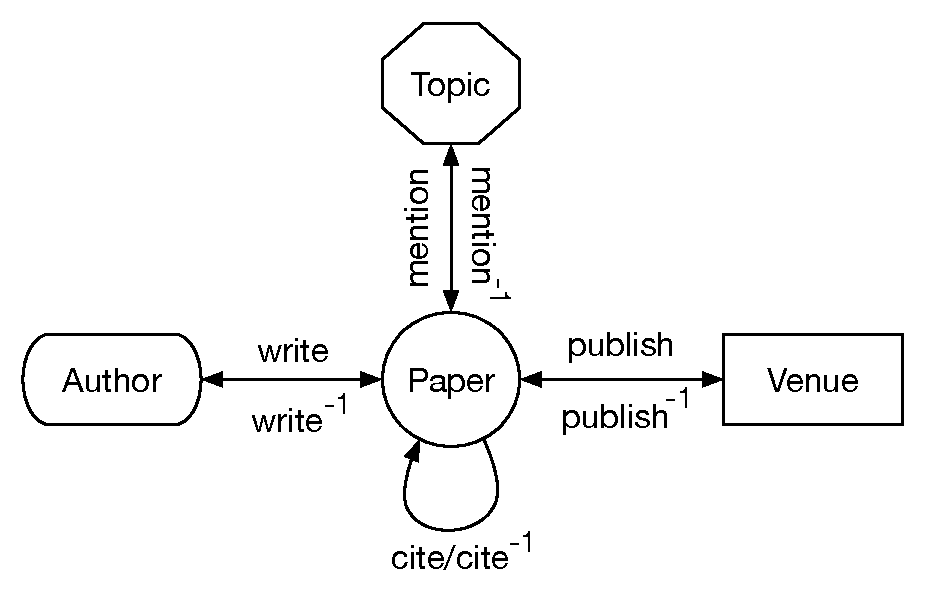
\includegraphics[width=0.4\textwidth]{figs/schema.pdf}
  \caption{Network schema for DBLP network.}\label{schema}
\end{figure}

\subsection{Meta path-based topology}

Similar to the notion of network schema that provides a meta structure for the network, a \textit{meta path} \cite{sun2011pathsim} provides a meta structure for paths between different nodes in the network. 

\begin{definition}[Meta path]
A meta path $\mathcal{P}$ is a path in the network schema graph $S_G = (\mathcal{A,R})$, denoted in the form of $\mathcal{P} = A_1 \xrightarrow{R_1} A_2... \xrightarrow{R_n} A_{n+1}$, as a sequence of links between node types, which defines a composite relationship between a node of type $A_1$ and one of type $A_{n+1}$. $\Box$
\end{definition}



\begin{example}
In the DBLP network, the co-author relationphip can be described with the meta path $A\xrightarrow{write}P\xrightarrow{write^{-1}}A$ or in short form \textit{A--P--A}. Paths in thick solid lines in Figure \ref{sampleNetwork} correspond to \textit{A--P--V--P--A} meta paths between \textit{Max} and \textit{Ada}, indicating they published in the same venue, such as \textit{Max--P1--KDD--P3--Ada}. $\Box$

\end{example}

Each meta path indicates a different semantic for a path connecting two nodes, and defines a unique topology representing a special relation. For instance the relationship between two authors are different when they are co-authors (\textit{A--P--A}) versus one citing another's paper (\textit{A--P--P--A}).

\begin{figure}[t]
  \centering
      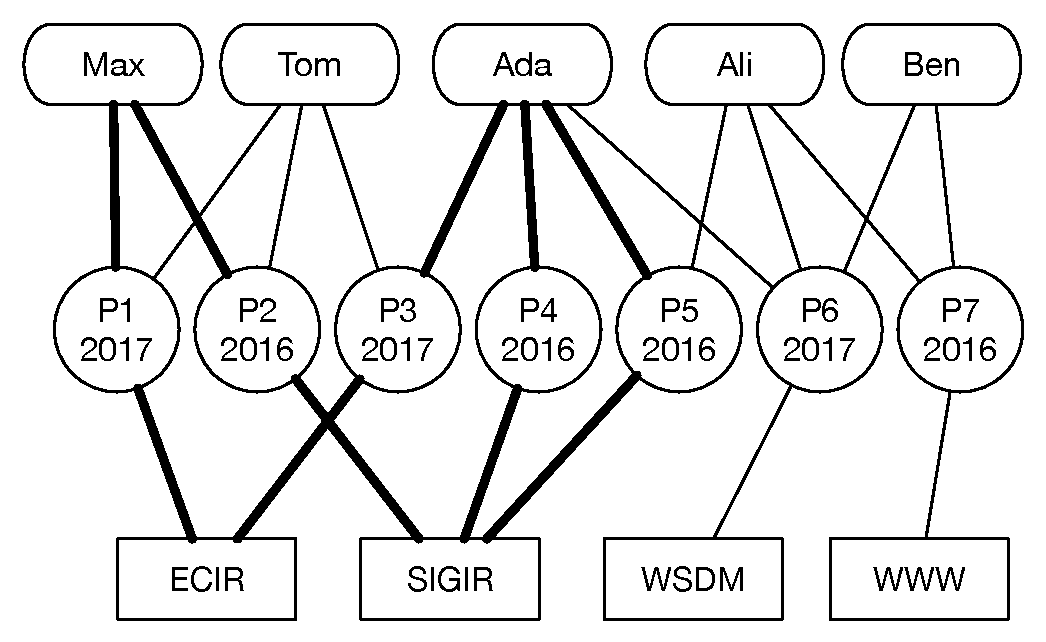
\includegraphics[width=0.4\textwidth]{figs/exampleSocialNetwork.pdf}
  \caption{An example of \textit{A--P--V--P--A} meta paths between two authors Max and Ada.}\label{sampleNetwork}
\end{figure}



%By checking the existing topological features defined in homogeneous networks, we can find that both the neighbor set-based features and path-based features can be generalized in heterogeneous information networks, by considering paths following different meta paths. For example, if we treat each type of neighbors separately and extend the immediate neighbors to n-hop neighbors (i.e., the distance between one object and its neighbors are n), the common neighbor feature between two authors is then becoming the count of paths between the two authors following different meta paths. For path-based features, such as Katz, it can be extended as a combination of paths following different meta paths. 


\begin{table*}[h]
\centering
\caption{Notations and their description.\amin{Needs to be updated according to the latest version.}\amin{This table will be later removed to to page space limit.}}
\label{table_notations}
\begin{tabular}{|c|l|} \hline
\textbf{Notation} & \textbf{Description} \\ \hline
$\mathcal{P}$, $p$  & Meta path and path \\ \hline
$k$ & The dimension of latent features \\ \hline
$G_\tau$ & Graph $G$ at time $\tau$  \\ \hline
$\hat{G}_\tau$ & Predicted graph $G$ at time $\tau$  \\ \hline
$Z_\tau$ & low rank $k$-dimensional latent space representation matrix for $G_\tau$ \\ \hline

%We will use capital variables (e.g. X) to denote matrices and lower-case variables (e.g. x) to denote vectors.We will use xi to mean the ith row of the matrix X. The Frobenius norm of the matrix X is denoted by ||X||2F = i||xi||22.

\end{tabular}
\end{table*}

